% Created by tikzDevice version 0.12.6 on 2026-05-14 20:42:38
% !TEX encoding = UTF-8 Unicode
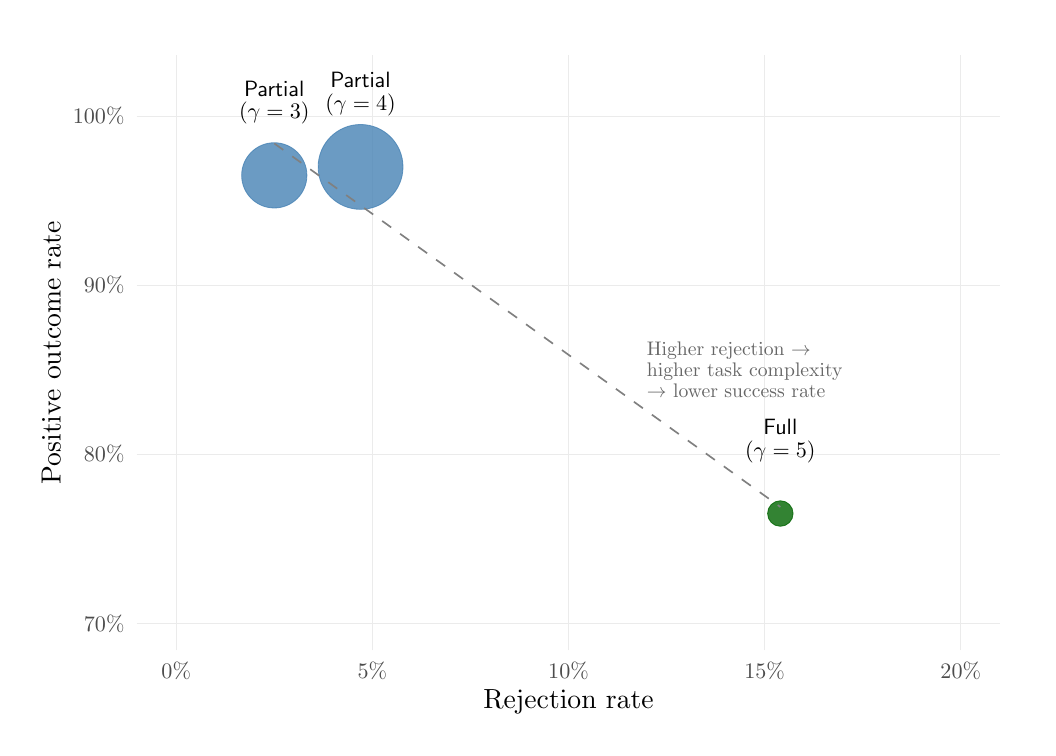
\begin{tikzpicture}[x=1pt,y=1pt]
\definecolor{fillColor}{RGB}{255,255,255}
\path[use as bounding box,fill=fillColor,fill opacity=0.00] (0,0) rectangle (361.35,252.94);
\begin{scope}
\path[clip] (  0.00,  0.00) rectangle (361.35,252.94);
\definecolor{fillColor}{RGB}{255,255,255}

\path[fill=fillColor] ( -0.00, -0.00) rectangle (361.35,252.94);
\end{scope}
\begin{scope}
\path[clip] ( 39.49, 27.90) rectangle (351.35,242.94);
\definecolor{drawColor}{gray}{0.92}

\path[draw=drawColor,line width= 0.5pt,line join=round] ( 39.49, 37.67) --
	(351.35, 37.67);

\path[draw=drawColor,line width= 0.5pt,line join=round] ( 39.49, 98.76) --
	(351.35, 98.76);

\path[draw=drawColor,line width= 0.5pt,line join=round] ( 39.49,159.86) --
	(351.35,159.86);

\path[draw=drawColor,line width= 0.5pt,line join=round] ( 39.49,220.95) --
	(351.35,220.95);

\path[draw=drawColor,line width= 0.5pt,line join=round] ( 53.67, 27.90) --
	( 53.67,242.94);

\path[draw=drawColor,line width= 0.5pt,line join=round] (124.55, 27.90) --
	(124.55,242.94);

\path[draw=drawColor,line width= 0.5pt,line join=round] (195.42, 27.90) --
	(195.42,242.94);

\path[draw=drawColor,line width= 0.5pt,line join=round] (266.30, 27.90) --
	(266.30,242.94);

\path[draw=drawColor,line width= 0.5pt,line join=round] (337.17, 27.90) --
	(337.17,242.94);
\definecolor{drawColor}{RGB}{0,100,0}
\definecolor{fillColor}{RGB}{0,100,0}

\path[draw=drawColor,draw opacity=0.80,line width= 0.3pt,line join=round,line cap=round,fill=fillColor,fill opacity=0.80] (271.97, 77.38) circle (  4.61);
\definecolor{drawColor}{RGB}{70,130,180}
\definecolor{fillColor}{RGB}{70,130,180}

\path[draw=drawColor,draw opacity=0.80,line width= 0.3pt,line join=round,line cap=round,fill=fillColor,fill opacity=0.80] (120.29,202.62) circle ( 15.32);

\path[draw=drawColor,draw opacity=0.80,line width= 0.3pt,line join=round,line cap=round,fill=fillColor,fill opacity=0.80] ( 89.11,199.57) circle ( 11.78);
\definecolor{drawColor}{RGB}{0,0,0}

\node[text=drawColor,anchor=base,inner sep=0pt, outer sep=0pt, scale=  0.80] at (271.97,105.93) {$\mathsf{Full}$};

\node[text=drawColor,anchor=base,inner sep=0pt, outer sep=0pt, scale=  0.80] at (271.97, 97.80) {($\gamma=5$)};

\node[text=drawColor,anchor=base,inner sep=0pt, outer sep=0pt, scale=  0.80] at (120.29,231.17) {$\mathsf{Partial}$};

\node[text=drawColor,anchor=base,inner sep=0pt, outer sep=0pt, scale=  0.80] at (120.29,223.04) {($\gamma=4$)};

\node[text=drawColor,anchor=base,inner sep=0pt, outer sep=0pt, scale=  0.80] at ( 89.11,228.11) {$\mathsf{Partial}$};

\node[text=drawColor,anchor=base,inner sep=0pt, outer sep=0pt, scale=  0.80] at ( 89.11,219.99) {($\gamma=3$)};
\definecolor{drawColor}{gray}{0.50}

\path[draw=drawColor,line width= 0.6pt,dash pattern=on 4pt off 4pt ,line join=round] ( 89.11,211.11) --
	( 91.42,209.45) --
	( 93.74,207.78) --
	( 96.05,206.12) --
	( 98.37,204.46) --
	(100.68,202.80) --
	(103.00,201.13) --
	(105.31,199.47) --
	(107.62,197.81) --
	(109.94,196.15) --
	(112.25,194.48) --
	(114.57,192.82) --
	(116.88,191.16) --
	(119.20,189.49) --
	(121.51,187.83) --
	(123.83,186.17) --
	(126.14,184.51) --
	(128.46,182.84) --
	(130.77,181.18) --
	(133.09,179.52) --
	(135.40,177.86) --
	(137.72,176.19) --
	(140.03,174.53) --
	(142.35,172.87) --
	(144.66,171.20) --
	(146.97,169.54) --
	(149.29,167.88) --
	(151.60,166.22) --
	(153.92,164.55) --
	(156.23,162.89) --
	(158.55,161.23) --
	(160.86,159.57) --
	(163.18,157.90) --
	(165.49,156.24) --
	(167.81,154.58) --
	(170.12,152.91) --
	(172.44,151.25) --
	(174.75,149.59) --
	(177.07,147.93) --
	(179.38,146.26) --
	(181.69,144.60) --
	(184.01,142.94) --
	(186.32,141.28) --
	(188.64,139.61) --
	(190.95,137.95) --
	(193.27,136.29) --
	(195.58,134.62) --
	(197.90,132.96) --
	(200.21,131.30) --
	(202.53,129.64) --
	(204.84,127.97) --
	(207.16,126.31) --
	(209.47,124.65) --
	(211.79,122.99) --
	(214.10,121.32) --
	(216.42,119.66) --
	(218.73,118.00) --
	(221.04,116.33) --
	(223.36,114.67) --
	(225.67,113.01) --
	(227.99,111.35) --
	(230.30,109.68) --
	(232.62,108.02) --
	(234.93,106.36) --
	(237.25,104.70) --
	(239.56,103.03) --
	(241.88,101.37) --
	(244.19, 99.71) --
	(246.51, 98.04) --
	(248.82, 96.38) --
	(251.14, 94.72) --
	(253.45, 93.06) --
	(255.77, 91.39) --
	(258.08, 89.73) --
	(260.39, 88.07) --
	(262.71, 86.41) --
	(265.02, 84.74) --
	(267.34, 83.08) --
	(269.65, 81.42) --
	(271.97, 79.75);
\definecolor{drawColor}{gray}{0.40}

\node[text=drawColor,anchor=base west,inner sep=0pt, outer sep=0pt, scale=  0.71] at (223.77,134.54) {Higher rejection $\rightarrow$};

\node[text=drawColor,anchor=base west,inner sep=0pt, outer sep=0pt, scale=  0.71] at (223.77,126.86) {higher task complexity};

\node[text=drawColor,anchor=base west,inner sep=0pt, outer sep=0pt, scale=  0.71] at (223.77,119.18) {$\rightarrow$ lower success rate};
\end{scope}
\begin{scope}
\path[clip] (  0.00,  0.00) rectangle (361.35,252.94);
\definecolor{drawColor}{gray}{0.30}

\node[text=drawColor,anchor=base east,inner sep=0pt, outer sep=0pt, scale=  0.80] at ( 34.99, 34.92) {70\%};

\node[text=drawColor,anchor=base east,inner sep=0pt, outer sep=0pt, scale=  0.80] at ( 34.99, 96.01) {80\%};

\node[text=drawColor,anchor=base east,inner sep=0pt, outer sep=0pt, scale=  0.80] at ( 34.99,157.10) {90\%};

\node[text=drawColor,anchor=base east,inner sep=0pt, outer sep=0pt, scale=  0.80] at ( 34.99,218.20) {100\%};
\end{scope}
\begin{scope}
\path[clip] (  0.00,  0.00) rectangle (361.35,252.94);
\definecolor{drawColor}{gray}{0.30}

\node[text=drawColor,anchor=base,inner sep=0pt, outer sep=0pt, scale=  0.80] at ( 53.67, 17.89) {0\%};

\node[text=drawColor,anchor=base,inner sep=0pt, outer sep=0pt, scale=  0.80] at (124.55, 17.89) {5\%};

\node[text=drawColor,anchor=base,inner sep=0pt, outer sep=0pt, scale=  0.80] at (195.42, 17.89) {10\%};

\node[text=drawColor,anchor=base,inner sep=0pt, outer sep=0pt, scale=  0.80] at (266.30, 17.89) {15\%};

\node[text=drawColor,anchor=base,inner sep=0pt, outer sep=0pt, scale=  0.80] at (337.17, 17.89) {20\%};
\end{scope}
\begin{scope}
\path[clip] (  0.00,  0.00) rectangle (361.35,252.94);
\definecolor{drawColor}{RGB}{0,0,0}

\node[text=drawColor,anchor=base,inner sep=0pt, outer sep=0pt, scale=  1.00] at (195.42,  6.94) {Rejection rate};
\end{scope}
\begin{scope}
\path[clip] (  0.00,  0.00) rectangle (361.35,252.94);
\definecolor{drawColor}{RGB}{0,0,0}

\node[text=drawColor,rotate= 90.00,anchor=base,inner sep=0pt, outer sep=0pt, scale=  1.00] at ( 11.89,135.42) {Positive outcome rate};
\end{scope}
\end{tikzpicture}
